\documentclass[journal=jpcbfk]{achemso}

\usepackage[version=3]{mhchem}
\usepackage[T1]{fontenc}
\newcommand*\mycommand[1]{\texttt{\emph{#1}}}
\newcommand{\todo}[1]{\textcolor{red}{#1}}

\usepackage{rotating}
\usepackage{upgreek}				
\usepackage{xcolor}
\usepackage{booktabs}
\usepackage{multirow}
\usepackage{lmodern}
\usepackage{microtype}
\usepackage{soul}
\usepackage{xr}

\makeatletter
\newcommand*{\addFileDependency}[1]{% argument=file name and extension
  \typeout{(#1)}
  \@addtofilelist{#1}
  \IfFileExists{#1}{}{\typeout{No file #1.}}
}
\makeatother

\newcommand*{\myexternaldocument}[1]{%
    \externaldocument{#1}%
    \addFileDependency{#1.tex}%
    \addFileDependency{#1.aux}%
    \addFileDependency{MANUSCRIPT/#1.tex}%
    \addFileDependency{MANUSCRIPT/#1.aux}%
}

\externaldocument{manuscript}

\author{Fernando Favela-Rosales}
\affiliation{Departamento de F\'isica, Centro de Investigaci\'on y de Estudios Avanzados del IPN, Apartado Postal 14-740, 07000 M\'exico D.F., M\'exico}
%
\author{Peter Heftberger}
\affiliation{Institute of Molecular Biosciences, Biophysics Division, NAWI Graz, University of Graz, Graz 8010, Austria}
%
\author{Matti Javanainen}
\email{matti.javanainen@helsinki.fi}
\affiliation{Institute of Organic Chemistry and Biochemistry,
Academy of Sciences of the Czech Republic, 
Prague 6, Czech Republic}
\alsoaffiliation{Institute of Biotechnology, University of Helsinki}
%
\author{Jesper J. Madsen}
\affiliation{Department of Global Health, College of Public Health}
\alsoaffiliation{University of South Florida}
%
\author{Josef Melcr}
\affiliation{Institute of Organic Chemistry and Biochemistry,
Academy of Sciences of the Czech Republic, 
Prague 6, Czech Republic}
%
\author{Markus Miettinen}
\affiliation{MPI}
%
\author{O. H. Samuli Ollila}
\email{samuli.ollila@helsinki.fi}
\affiliation{Institute of Organic Chemistry and Biochemistry,
Academy of Sciences of the Czech Republic, 
Prague 6, Czech Republic}
\alsoaffiliation{Institute of Biotechnology, University of Helsinki}
%
\author{Georg Pabst}
\affiliation{Institute of Molecular Biosciences, Biophysics Division, NAWI Graz, University of Graz, Graz 8010, Austria}
\alsoaffiliation{BioTechMed-Graz, Graz 8010, Austria}
%
\author{Thomas Piggot}
\affiliation{School of Chemistry, University of Southamptaon, Southampton SO17 1BJ, United Kingdom}
\alsoaffiliation{Chemical Biological and Radiological Sciences, Defence Science and Technology Laboratory, Porton Down, Salisbury, Wiltshire SP4 0JQ, United Kingdom}

\SectionNumbersOn

\renewcommand{\thetable}{S\arabic{table}}%
\renewcommand{\thefigure}{S\arabic{figure}}%
\renewcommand{\thesection}{S\arabic{section}}%
\renewcommand{\thepage}{S\arabic{page}}%


\title{SUPPLEMENTARY INFORMATION FOR\\ 
    NMRlipids III: Lipid--Cholesterol Interactions in Atomistic Resolution Molecular Dynamics Simulations}

\begin{document}

\tableofcontents

\section{Simulation Parameters}

The force field specific simulation parameters used for each force field are listed in Table~\ref{SItab:params}. The parameter input files (\texttt{.mdp}) are provided in the Zenodo portal (links in the main text). For all simulations, we used an integration time step of 2~fs and the leap-frog integrator of GROMACS. The isothermal--isobaric (NPT) ensemble was used with a temperature of 298~K and a pressure of 1~bar. All simulations were 1~\textmu{}s long, and trajectories were written every 1~ns. The P-LINCS constraint algorithm \cite{hess97,hess07} was used for the bonds noted in Table~\ref{SItab:params}. 

\begin{sidewaystable}[]
\begin{center}
    \caption{\label{SItab:params}%
    Simulation parameters used for different force fields.
    }
    \begin{tabular}{lcccc}
    \toprule
    \textbf{Parameter} & \textbf{CHARMM36} & \textbf{Slipids} & \textbf{Lipid17} & \textbf{MacRog} \\
    \midrule % NB interactions
    Neighbour list type & Verlet \cite{pall2013flexible} & Verlet \cite{pall2013flexible} & Verlet \cite{pall2013flexible} & Verlet \cite{pall2013flexible} \\
    Long-range electrostatics & PME & PME & PME & PME \\
    LJ cut-off & 1.2~nm & 1.4~nm & 0.9~nm & 1.0~nm \\
    LJ modifier & Force switch 1.0--1.2~nm & -- & -- & -- \\
    Dispersion correction & -- & Energy \& pressure \cite{shirts2007accurate} & Energy \& pressure \cite{shirts2007accurate} & Energy \& pressure \cite{shirts2007accurate} \\
    \midrule % P/T control
    Thermostat & Nos\'{e}--Hoover \cite{hoover85,nose84} & Stochastic rescaling \cite{bussi07} & Nos\'{e}--Hoover \cite{hoover85,nose84} & Stochastic rescaling \cite{bussi07} \\
    Time constant ($T$) & 1~ps & 0.5~ps & 1~ps & 0.1~ps \\
    Coupling groups & Lipids \& water & Lipids \& water & Lipids \& water & Lipids \& water \\
    Barostat & Parrinello--Rahman \cite{parrinello1981polymorphic} & Berendsen \cite{berendsen1984molecular} & Parrinello--Rahman \cite{parrinello1981polymorphic} & Parrinello--Rahman \cite{parrinello1981polymorphic} \\
    Coupling type ($P$) & semi-isotropic & semi-isotropic & semi-isotropic & semi-isotropic \\
    Time constant ($P$) & 5~ps & 10~ps & 5~ps & 4~ps\\
    Compressibility & 4.5$\cdot$10$^{-5}$~1/bar & 4.5$\cdot$10$^{-5}$~1/bar & 4.5$\cdot$10$^{-5}$~1/bar & 4.5$\cdot$10$^{-5}$~1/bar \\
    \midrule % Constraints
    Constraints & Bonds with H & All bonds & Bonds with H & All bonds \\
    \midrule 
    Water model & TIPS3P \cite{durell1994solvent}  & TIP3P \cite{jorgensen83} & TIP3P \cite{jorgensen83} & TIP3P \cite{jorgensen83} \\
    FF Source & CHARMM-GUI & CHARMM-GUI & CHARMM-GUI & Refs.~\citenum{kulig2016cis} \& \citenum{macrogpopc} \\
    Parameter source & CHARMM-GUI & Slipids website & CHARMM-GUI & Refs.~\citenum{kulig2016cis} \& \citenum{macrogpopc} \\
    \bottomrule
    \end{tabular}
\end{center}
\end{sidewaystable}

\clearpage

\section{Additional Results}

\subsection{Scattering Intensities}

\begin{figure}[htb!]
    \centering
    \includegraphics[width=0.49\linewidth]{FIGS/scatt0.pdf}
    \includegraphics[width=0.49\linewidth]{FIGS/scatt5.pdf}\\
    \includegraphics[width=0.49\linewidth]{FIGS/scatt10.pdf}
    \includegraphics[width=0.49\linewidth]{FIGS/scatt15.pdf}\\
    \includegraphics[width=0.49\linewidth]{FIGS/scatt20.pdf}
    \includegraphics[width=0.49\linewidth]{FIGS/scatt25.pdf}
    \caption{Scattering intensities from X-ray scattering experiments with various concentrations of cholesterol. More data are shown in the next figure.}
    \label{SIfig:scattering1}
\end{figure}

\begin{figure}[htb!]
    \centering
    \includegraphics[width=0.49\linewidth]{FIGS/scatt30.pdf}
    \includegraphics[width=0.49\linewidth]{FIGS/scatt35.pdf}\\
    \includegraphics[width=0.49\linewidth]{FIGS/scatt40.pdf}
    \includegraphics[width=0.49\linewidth]{FIGS/scatt45.pdf}\\
    \includegraphics[width=0.49\linewidth]{FIGS/scatt50.pdf}
    \caption{Scattering intensities from X-ray scattering experiments with various concentrations of cholesterol. More data are shown in the previous figure.}
    \label{SIfig:scattering2}
\end{figure}

\subsection{Form Factors \& Electron Density Profiles}

\begin{figure}[htb!]
    \centering
    \includegraphics[width=0.86\linewidth]{../FIGS/scattering.pdf}
    \caption{\label{SIfig:scattering}%
     \textbf{Scattering intensities as a function of scattering vector from experiments and simulations.} Each of the profiles is shifted vertically with respect to the previous one, by 1 for the experimental profiles and by 50 for the computational ones. The minima are marked by filled circles to guide the eye.
    }
\end{figure}

\begin{figure}[htb!]
    \centering
    \includegraphics[width=8.7cm]{../FIGS/ffminima.pdf}
    \caption{\label{SIfig:ffminima}%
    \textbf{Effecf of CHOL on the location of the first two minima in the form factor.}
    The minima are extracted from the form factors interpolated to all CHOL concentrations (Fig.~\ref{SIfig:scattering}) from experiment and simulation with the \texttt{findpeaks} function in Matlab.
    }
\end{figure}

\begin{figure}[htb!]
    \centering
    \includegraphics[width=\linewidth]{../FIGS/densityprofiles.pdf}
    \caption{\label{SIfig:densprofs}%
    \textbf{Electron density profiles.}
    Each of the profiles is shifted vertically with respect to the previous one by 100 units.
    }
\end{figure}

\clearpage
\subsection{Order Parameters}

\begin{figure}[htb!]
    \centering
    \includegraphics[width=0.9\linewidth]{../FIGS/palmitate.pdf}
    \caption{\label{SIfig:palmitate}%
     \textbf{Effect of cholesterol on the acyl chain order parameters of the POPC $sn$-1 (palmitate) chain.}
     The legend at the top corresponds to all simulations, and the one at the bottom to the experiments.
    }
\end{figure}

\begin{figure}[htb!]
    \centering
    \includegraphics[width=0.9\linewidth]{../FIGS/oleate.pdf}
    \caption{\label{SIfig:oleate}%
     \textbf{Effect of cholesterol on the acyl chain order parameters of the POPC $sn$-2 (oleate) chain.}
     The legend at the top corresponds to all simulations, and the one at the bottom to the experiments. Since the order parameters measured for the two hydrogens bound to the C2 carbon differ, they are both shown in the plots.
    }
\end{figure}

\begin{figure}[htb!]
    \centering
    \includegraphics[width=\linewidth]{../FIGS/OP_headgroup.pdf}
    \caption{\label{SIfig:headgroups}%
     \textbf{The deviation of POPC head group parameters from experimental values as a function of CHOL concentration.}
    }
\end{figure}

\clearpage
\subsection{Dynamic Properties}

\begin{figure}[htb!]
    \centering
    \includegraphics[width=0.9\linewidth]{../FIGS/d_vs_size.pdf}
    \caption{\label{SIfig:dvssize}%
    \textbf{Dependence of lateral diffusion coefficients on simulation box size.} The values calculated for the lipid centres of mass with \texttt{gmx msd} after eliminating leaflet drift. The values for the three system sizes are shown as markers together with fits of Eq.~\eqref{eq:pbc}. The values extrapolated to infinite system sizes are also shown in the separate column. 
    }
\end{figure}

\begin{figure}[htb!]
    \centering
    \includegraphics[width=0.9\linewidth]{../FIGS/d_vs_chol.pdf}
    \caption{\label{SIfig:dvschol}%
     \textbf{Dependence of lateral diffusion coefficients on cholesterol concentration.} Data are shown for all system sizes; small (S), medium (M), and large (L). The values extrapolated to infinity are shown as well ($\infty$). Experimental measured at two hydration levels, 30 m-\% and 55-\% of water \cite{filippov2003effect,filippov2003influence}.
    }
\end{figure}

\clearpage
\subsection{Finite-Size Effects}

\begin{figure}[htb!]
    \centering
    \includegraphics[width=8.7cm]{../FIGS/apl_vs_size.pdf}
    \caption{\label{SIfig:aplvssize}%
     \textbf{Dependence of area per lipid on simulation box size.} Area per lipid is calculated by dividing the membrane area by the number of lipids in one leaflet. Error bars show standard error extracted using block averaging in \texttt{gmx analyze}.
    }
\end{figure}

\begin{figure}[htb!]
    \centering
    \includegraphics[width=\linewidth]{../FIGS/densityprofiles_size.pdf}
    \caption{\label{SIfig:densprofssize}%
    \textbf{Effect of system size on the density profiles.}
    Membrane undulations are larger in the larger systems, which leads to the smearing of the electron density profiles. Here, data are shown for CHARMM36 in the large (1024 POPC in total), medium (256 POPC in total), or small (64 POPC in total) systems. The experimental electron density profile is shown for comparison.
    }
\end{figure}

\clearpage
\subsection{Cholesterol Tilt}

\begin{figure}[htb!]
    \centering
    \includegraphics[width=8.7cm]{../FIGS/choltilt.pdf}
    \caption{\label{SIfig:choltilt}%
     \textbf{Effect of cholesterol concentration on the tilt of the cholesterol molecules.}
     The tilt is defined as the angle between the vector connecting the C3 and C17 carbons at the two ends of the rigid ring structure of cholesterol. The hydroxyl group is bound to C3 and the hydrocarbon chain to C17. The tilt distributions were gathered from the two leaflets, fitted with a Gamma distribution, and the mean values and standard deviations were extracted and shown here as the value and error estimate, respectively. The cholesterol concentration was identical between the simulations, but the points are horizontally slightly shifted for clarity.
    }
\end{figure}

\clearpage


\bibliography{refs.bib}

\end{document}


\section{CHARMM36 results from different simulation packages} \label{CHARMMprograms}
The results from CHARMM36 model for lipid bilayers from different 
simulation packages have been reported to give different results in
the literature \cite{piggot12,lee16}. The results are mainly
dependent on different Lennard-Jones cut-off settings, but
all the details are not quite understood. In this work we use
the results from Gromacs 5 with settings suggested to be optimal
by Gromacs webpage.~\todo{List these settings here or in SI.} We also compared the results from Gromacs 5 with
these settings to the results simulated with NAMD, OpenMM and literature
values. Based on comparison shown in Fig. \ref{programsCOMP}, we conclude
that Gromacs 5 with settings suggested in webpage gives consistent
results with the literature and other simulation packages. Thus these
results are used in the main body of the paper. However, order parameters
are slightly overestimated respected to the experiments also with these
settings. \\
\todo{Should be extend this discussion based on discussion at  https://github.com/NMRLipids/NmrLipidsCholXray/issues/4 ?}
 \begin{figure}[]
  \centering
  \includegraphics[width=8cm]{../FIGS/OrderParametersPROGRAMS.eps}

  \caption{\label{programsCOMP}
    Results for CHARMM36 model \cite{klauda10} from different simulation packages.
    Discussion going on at {\it https://github.com/NMRLipids/NmrLipidsCholXray/issues/4}.
  }
\end{figure}

\clearpage
\section{Order parameter slopes as a function of cholesterol}
 \begin{figure*}[]
  \centering
  \includegraphics[width=19cm]{../FIGS/slopesEXPERIMENT.pdf}
  \caption{\label{slopes}
    Slopes of order parameters as a function of cholesterol from experiments \cite{ferreira13}.
  }
\end{figure*}

 \begin{figure*}[]
  \centering
  \includegraphics[width=19cm]{../FIGS/slopesBERGER.pdf}
  \caption{\label{slopesberger}
    Slopes of order parameters as a function of cholesterol from Berger simulations.
  }
\end{figure*}

 \begin{figure*}[]
  \centering
  \includegraphics[width=19cm]{../FIGS/slopesCHARMM.pdf}
  \caption{\label{slopescharmm}
    Slopes of order parameters as a function of cholesterol from CHARMM36 simulations.
  }
\end{figure*}
 \begin{figure*}[]
  \centering
  \includegraphics[width=19cm]{../FIGS/slopesMACROG.pdf}
  \caption{\label{slopesmacrog}
    Slopes of order parameters as a function of cholesterol from MacRog simulations.
  }
\end{figure*}
 \begin{figure*}[]
  \centering
  \includegraphics[width=19cm]{../FIGS/slopesSLIPIDS.pdf}
  \caption{\label{slopesslipids}
    Slopes of order parameters as a function of cholesterol from Slipids simulations.
  }
\end{figure*}
 \begin{figure*}[]
  \centering
  \includegraphics[width=19cm]{../FIGS/slopesSLIPIDST310K.pdf}
  \caption{\label{slopesslipids310K}
    Slopes of order parameters as a function of cholesterol from Slipids simulations at 298 K.
  }
\end{figure*}


\clearpage
 \section{Effect of undulations on order parameters} \label{undulations}
 \todo{This should be written based on contributions in this issue:
   https://github.com/NMRLipids/NmrLipidsCholXray/issues/16
 }
 
% \begin{figure}[]
%  \centering
%  \includegraphics[width=8cm]{../FIGS/slopesBERGER.pdf}
%  \caption{\label{programsCOMP}
%    Slopes of order parameters as a function of cholesterol from Berger simulations.
%  }
%\end{figure}